% la-02-lineareqs.tex

\documentclass[xcolor=dvipsnames]{beamer}
\usepackage{teachbeamer}

\title{Linear Equations}
\subtitle{{\CourseNumber}, BCIT}

\author{\CourseName}

\date{September 17, 2018}

\begin{document}

\begin{frame}
  \titlepage
\end{frame}

\begin{frame}
  \frametitle{Systems of Linear Equations Introduced}
  Chaitali and Amulya go to a concession stand to buy fruit. Chaitali
  buys 5 bananas and 3 apples and spends \$13.50. Amulya buys 1 banana
  and 5 apples and spends 20 cents more than Chaitali. How much do
  bananas and apples cost at the concession stand?
\end{frame}

\begin{frame}
  \frametitle{Systems of Linear Equations Introduced}
  Chaitali and Amulya go to a concession stand to buy fruit. Chaitali
  buys 5 bananas and 3 apples and spends \$13.50. Amulya buys 1 banana
  and 5 apples and spends 20 cents more than Chaitali. How much do
  bananas and apples cost at the concession stand?
  \begin{equation}
    \label{eq:mohloogh}
    \begin{array}{rcrcl}
      5x&+&3y&=&13.5 \\
      x&+&5y&=&13.7
    \end{array}
  \end{equation}
\end{frame}

\begin{frame}
  \frametitle{What Is a System of Linear Equations?}
  \begin{equation}
    \label{eq:xaigeeke}
    \begin{array}{rcrcl}
      5x&+&3y&=&13.5 \\
      x&+&5y&=&13.7
    \end{array}
  \end{equation}
  This system of linear equations is the rule for the following set $S\subset\mathbb{R}\times\mathbb{R}$:
  \begin{equation}
    \label{eq:ahshohwa}
S=\{(x,y)\in\mathbb{R}\times\mathbb{R}|5x+3y=13.5\mbox{ and }x+5y=13.7\}
  \end{equation}
\end{frame}

\begin{frame}
  \frametitle{Solution Methods}
  \begin{equation}
    \label{eq:yeghahpi}
    \begin{array}{rcrcl}
      5x&+&3y&=&13.5 \\
      x&+&5y&=&13.7
    \end{array}
  \end{equation}
There are several ways to solve a system of equations like this. 
\begin{itemize}
\item Graphing
\item Substitution
\item Elimination
\item Using a Matrix
\end{itemize}
\end{frame}

\begin{frame}
  \frametitle{Graphing Method I}
  \begin{equation}
    \label{eq:oamaiwei}
    \begin{array}{rcrcl}
      5x&+&3y&=&13.5 \\
      x&+&5y&=&13.7
    \end{array}
  \end{equation}
is equivalent to
  \begin{equation}
    \label{eq:kaiquaeb}
    \begin{array}{rcl}
      y&=&-\frac{5}{3}x+\frac{9}{2} \\
      && \\
      y&=&-\frac{1}{5}x+\frac{137}{50}
    \end{array}
  \end{equation}
\end{frame}

\begin{frame}
  \frametitle{Graphing Method II}
  \begin{figure}[h]
    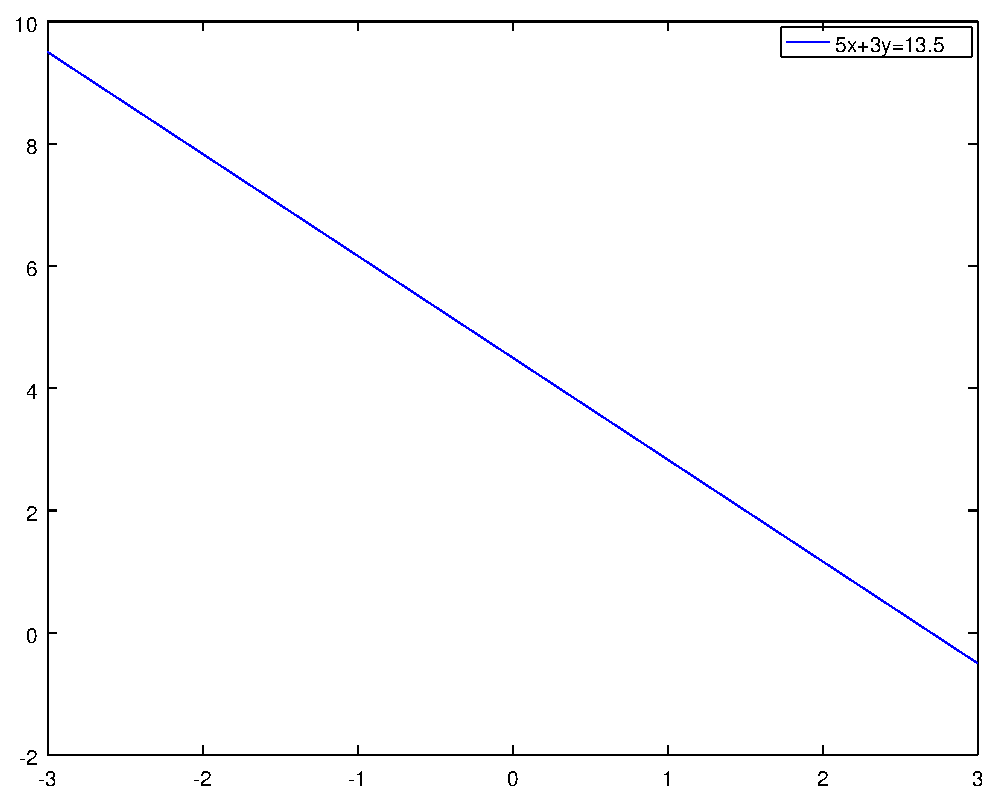
\includegraphics[scale=.6]{./diagrams/gm-03-SystemsEquations-01.eps}
  \end{figure}
\end{frame}

\begin{frame}
  \frametitle{Graphing Method III}
  \begin{figure}[h]
    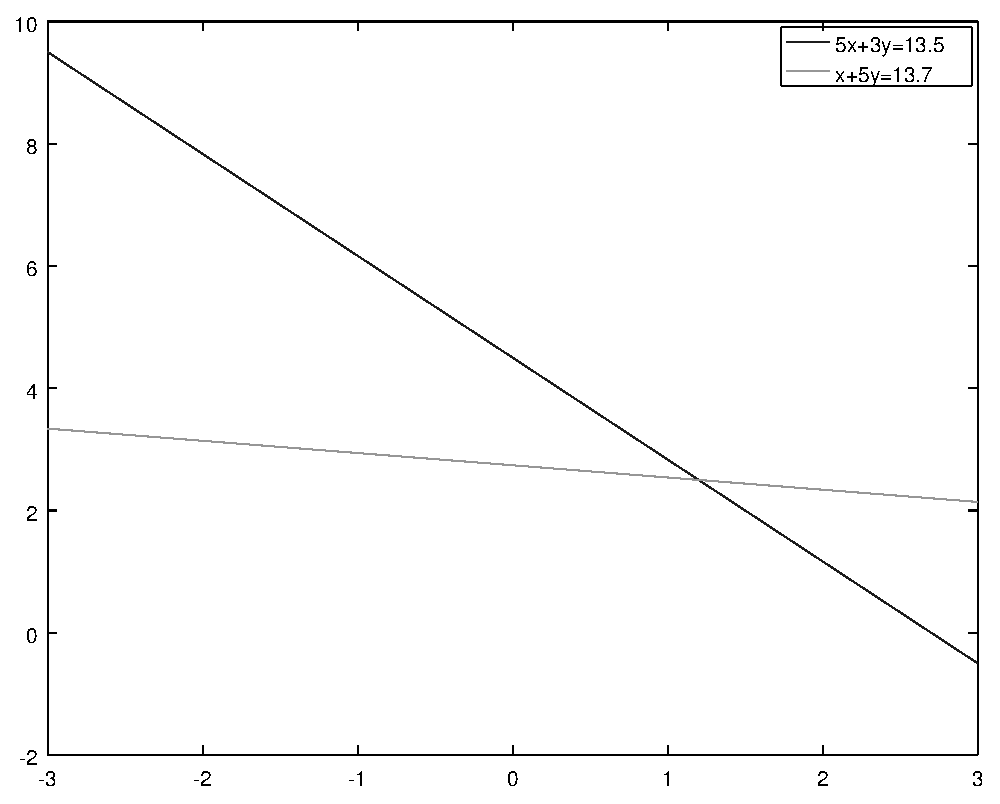
\includegraphics[scale=.6]{./diagrams/gm-03-SystemsEquations-02.eps}
  \end{figure}
\end{frame}

\begin{frame}
  \frametitle{Graphing Method IV}
  \begin{figure}[h]
    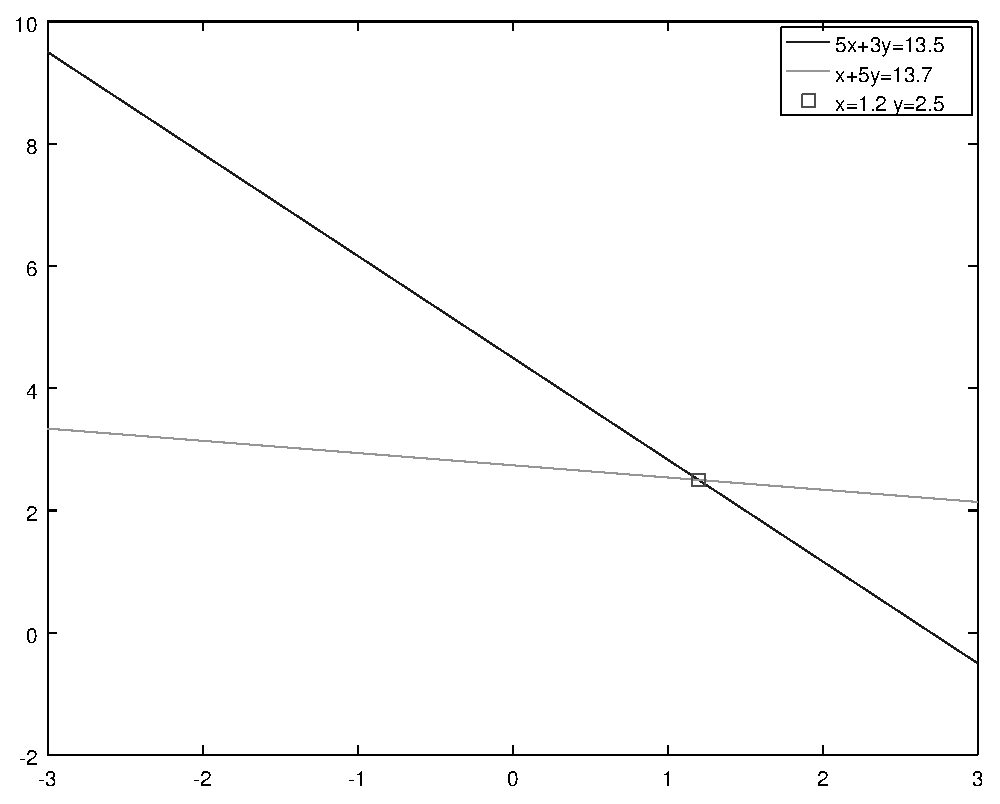
\includegraphics[scale=.6]{./diagrams/gm-03-SystemsEquations-03.eps}
  \end{figure}
\end{frame}

\begin{frame}
  \frametitle{Graphing Method V}
  \begin{figure}[h]
    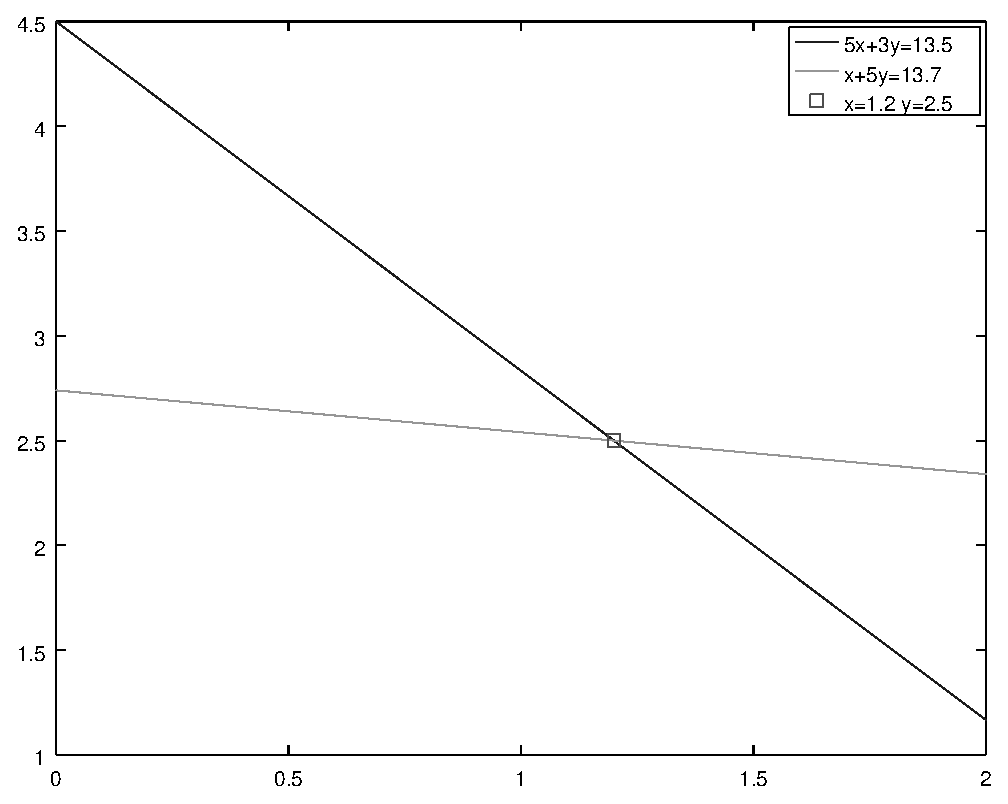
\includegraphics[scale=.6]{./diagrams/gm-03-SystemsEquations-04.eps}
  \end{figure}
\end{frame}

\begin{frame}
  \frametitle{Graphing Method Exercises}
Find a solution to these systems of linear equations by graphing them
and check your answer by substituting.
  \begin{equation}
    \label{eq:fiesebah}
    \begin{array}{rcrcl}
      7x&-&6y&=&19 \\
      -5x&+&2y&=&-9
    \end{array}
  \end{equation}
  \begin{equation}
    \label{eq:weaseiwa}
    \begin{array}{rcrcl}
      x&+&3y&=&12 \\
      11x&-&2y&=&27
    \end{array}
  \end{equation}
  \begin{equation}
    \label{eq:yaetooni}
    \begin{array}{rcrcl}
      \frac{1}{2}x&-&2y&=&\frac{9}{2} \\
      -\frac{5}{8}x&+&y&=&-\frac{15}{8}
    \end{array}
  \end{equation}
\end{frame}

\begin{frame}
  \frametitle{Substitution Method I}
  \begin{equation}
    \label{eq:jichoora}
    \begin{array}{rcrcl}
      5x&+&3y&=&13.5 \\
      x&+&5y&=&13.7
    \end{array}
  \end{equation}
The second equation yields $x=13.7-5y$. Use this to substitute in the
first equation
  \begin{equation}
    \label{eq:iewoobih}
5\cdot\alert{(13.7-5y)}+3y=13.5
  \end{equation}
therefore, $-22y=-55$ and $y=5/2$. Now substitute $y=5/2$ in the first
equation (you could just as well use the second equation), so
\begin{equation}
  \label{eq:phaiyahj}
  5x+3\cdot\frac{5}{2}=13.5
\end{equation}
which implies $x=1.2$. A banana costs \$1.20; an apple costs \$2.50.
\end{frame}

\begin{frame}
  \frametitle{Substitution Method Exercises}
Find a solution to these systems of linear equations by using the
substitution method.
  \begin{equation}
    \label{eq:waduifee}
    \begin{array}{rcrcl}
      7x&-&6y&=&19 \\
      -5x&+&2y&=&-9
    \end{array}
  \end{equation}
  \begin{equation}
    \label{eq:weiyushe}
    \begin{array}{rcrcl}
      x&+&3y&=&12 \\
      11x&-&2y&=&27
    \end{array}
  \end{equation}
  \begin{equation}
    \label{eq:jiadaush}
    \begin{array}{rcrcl}
      \frac{1}{2}x&-&2y&=&\frac{9}{2} \\
      -\frac{5}{8}x&+&y&=&-\frac{15}{8}
    \end{array}
  \end{equation}
\end{frame}

\begin{frame}
  \frametitle{Elimination Method I}
  \begin{equation}
    \label{eq:ohneirae}
    \begin{array}{rcrcl}
      5x&+&3y&=&13.5 \\
      x&+&5y&=&13.7
    \end{array}
  \end{equation}
is equivalent to
  \begin{equation}
    \label{eq:wahheedo}
    \begin{array}{rcrcl}
      5x&+&3y&=&13.5 \\
      5x&+&25y&=&68.5
    \end{array}
  \end{equation}
\end{frame}

\begin{frame}
  \frametitle{Elimination Method II}
  \begin{equation}
    \label{eq:zeegheir}
    \begin{array}{rcrcl}
      5x&+&3y&=&13.5 \\
      5x&+&25y&=&68.5
    \end{array}
  \end{equation}
implies
  \begin{equation}
    \label{eq:ooleeyae}
(5x+3y)-(5x+25y)=13.5-68.5
  \end{equation}
therefore, $-22y=-55$ and $y=5/2$. Now substitute $y=5/2$ in the first
equation (you could just as well use the second equation), so
\begin{equation}
  \label{eq:ieghoisa}
  5x+3\cdot\frac{5}{2}=13.5
\end{equation}
which implies $x=1.2$. A banana costs \$1.20; an apple costs \$2.50.
\end{frame}

\begin{frame}
  \frametitle{Elimination Method Exercises}
Find a solution to these systems of linear equations by using the
elimination method.
  \begin{equation}
    \label{eq:eighilai}
    \begin{array}{rcrcl}
      7x&-&6y&=&19 \\
      -5x&+&2y&=&-9
    \end{array}
  \end{equation}
  \begin{equation}
    \label{eq:thidaitu}
    \begin{array}{rcrcl}
      x&+&3y&=&12 \\
      11x&-&2y&=&27
    \end{array}
  \end{equation}
  \begin{equation}
    \label{eq:ohkaicux}
    \begin{array}{rcrcl}
      \frac{1}{2}x&-&2y&=&\frac{9}{2} \\
      -\frac{5}{8}x&+&y&=&-\frac{15}{8}
    \end{array}
  \end{equation}
\end{frame}

\begin{frame}
  \frametitle{Matrices and Systems of Linear Equations I}
Remember our system of linear equations. 
  \begin{equation}
    \label{eq:ahgohcoh}
    \begin{array}{rcrcl}
      5x & + & 3y & = & 13.5 \\
      x  & + & 5y & = & 13.7
    \end{array}
  \end{equation}
In matrix notation, we can write
  \begin{equation}
    \label{eq:neithohn}
  \left[\begin{array}{cc}
5        & 3                 \\
 1       & 5
  \end{array}\right]\cdot
  \left[\begin{array}{c}
 x                 \\
 y
  \end{array}\right]=
  \left[\begin{array}{c}
13.5                 \\
13.7
  \end{array}\right]\notag
  \end{equation}
\end{frame}

\begin{frame}
  \frametitle{Matrices and Systems of Linear Equations II}
Let's call these three matrices $A,v,b$ respectively. $A$ and $b$ are
provided, and we are looking for $v$. If we had $A^{-1}$, we could go
from
\begin{equation}
  \label{eq:baixieda}
  Av=b
\end{equation}
to
\begin{equation}
  \label{eq:maethung}
  A^{-1}Av=A^{-1}b
\end{equation}
which is the same as
\begin{equation}
  \label{eq:leighuga}
  v=A^{-1}b
\end{equation}
\end{frame}

\begin{frame}
  \frametitle{Matrix Row Operations}
  Another method to find the inverse of a matrix is using
  \alert{matrix row operations}. There are three matrix row
  operations.
\begin{itemize}
\item \alert{Row Switching} means you are allowed to switch two rows,
  for example $R_{1}\leftrightarrow{}R_{2}$
\item \alert{Row Multiplication} means you are allowed to multiply all
  elements of a row by a real non-zero number, for example
  $\frac{2}{5}R_{2}\rightarrow{}R_{2}$
\item \alert{Row Addition} means you are allowed to add one row to
  another and then replace one of the original rows by the sum of the
  two rows, for example $R_{1}+R_{2}\rightarrow{}R_{1}$
\end{itemize}
Row multiplication and row addition are often used together, for
example $\frac{7}{8}R_{1}-R_{3}\rightarrow{}R_{3}$.
\end{frame}

\begin{frame}
  \frametitle{Matrix Row Operations}
To find the inverse of a square matrix, we combine $A$ and $I$
  \begin{equation}
    \label{eq:aurohbac}
  \left[\begin{array}{cccc}
 5 & 3 & 1 & 0 \\
 1 & 5 & 0 & 1
  \end{array}\right]\notag
  \end{equation}
and apply matrix row operations until we get
  \begin{equation}
    \label{eq:nahshooh}
  \left[\begin{array}{cccc}
 1 & 0 & x & y \\
 0 & 1 & z & w
  \end{array}\right]\notag
  \end{equation}
where
  \begin{equation}
    \label{eq:aecocaeh}
  A^{-1}=\left[\begin{array}{cc}
 x & y  \\
 z & w 
  \end{array}\right]\notag
  \end{equation}
\end{frame}

\begin{frame}
  \frametitle{Inverse Example}
For our example,
  \begin{equation}
    \label{eq:weeraesh}
  \left[\begin{array}{cccc}
 5    & 3     & 1     & 0     \\
 1    & 5     & 0     & 1
  \end{array}\right]\longrightarrow
  \left[\begin{array}{cccc}
 25/3 & 5     & 5/3   & 0     \\
 1    & 5     & 0     & 1
        \end{array}\right]\longrightarrow\notag
\end{equation}
  \begin{equation}
  \left[\begin{array}{cccc}
 22/3 & 0     & 5/3   & -1    \\
 1    & 5     & 0     & 1
  \end{array}\right]\longrightarrow\notag
\end{equation}
  \begin{equation}
    \label{eq:ieyoongu}
  \left[\begin{array}{cccc}
 22/3 & 0     & 5/3   & -1    \\
 22/3 & 110/3 & 0     & 22/3
  \end{array}\right]\longrightarrow
  \left[\begin{array}{cccc}
 22/3 & 0     & 5/3   & -1    \\
 0    & 110/3 & -5/3  & 25/3
  \end{array}\right]\longrightarrow\notag
\end{equation}
  \begin{equation}
    \label{eq:ephoopha}
  \left[\begin{array}{cccc}
 1    & 0     & 5/22  & -3/22 \\
 0    & 1     & -1/22 & 5/22
  \end{array}\right]\notag
  \end{equation}
\end{frame}

\begin{frame}
  \frametitle{Inverse Example}
  For step 1, we multiplied the first row by $5/3$ (row
  multiplication). For step 2, we subtracted the second row from the
  first row and replaced the first row by the result (row addition).
  For step 3, we multiplied the second row by $22/3$ (row
  multiplication). For step 4, we subtracted the first row from the
  second row and replaced the second row by the result (row addition).
  For the last step, we multiplied the first row by $3/22$ and the
  second row by $3/110$ (row multiplication applied twice).
\end{frame}

\begin{frame}
  \frametitle{Matrices and Systems of Linear Equations III}
Thus,
\begin{equation}
  \label{eq:oogeujie}
  A^{-1}=\left[\begin{array}{cc}
 5/22  & -3/22 \\
 -1/22 & 5/22
               \end{array}\right]=\frac{1}{22}\cdot\left[
               \begin{array}{cc}
                 5 & -3 \\
                 -1 & 5
               \end{array}\right]\notag
\end{equation}
and
\begin{equation}
  \label{eq:seeleeje}
  v=A^{-1}b=\left[\begin{array}{cc}
 5/22  & -3/22 \\
 -1/22 & 5/22
  \end{array}\right]\cdot
\left[\begin{array}{c}
 13.5   \\
 13.7  
  \end{array}\right]=\left[\begin{array}{c}
 1.2   \\
 2.5  
  \end{array}\right]\notag
\end{equation}
The method combining $A$ and $I$ to form, by elementary row
operations, $I$ and $A^{-1}$ works because the total effect of the
elementary row operations is left-multiplication by $A^{-1}$. This
turns $A$ into $I$ and $I$ into $A^{-1}$. 
\end{frame}

% The following exercises are from http://www.algebralab.org/practice/practice.aspx?file=Word_ApplicationProblemFor3EquationsWith3Variables.xml

\begin{frame}
  \frametitle{System of Three Linear Equations Word Problems}
  {\ubung} Marina had \$24,500 to invest. She divided the money into
  three different accounts. At the end of the year, she had made
  \$1,300 in interest. The annual yield on each of the three accounts
  was 4\%, 5.5\%, and 6\%. If the amount of money in the 4\% account
  was four \%times the amount of money in the 5.5\% account, how much
  had she \%placed in each account?
\end{frame}

\begin{frame}
  \frametitle{System of Three Linear Equations Word Problems}
  {\ubung} The currents running through an electrical system are given
  by the following system of equations. The three currents $I_{1},I_{2},I_{3}$
  are measured in amps. Solve the system to find the currents in this
  circuit.
  \begin{align}
    \label{eq:oemeyeib}
    \begin{array}{clclclc}
    I_{1} & + & 2I_{2} & - & I_{3} & = & 0.425 \\
    3I_{1} & - & I_{2} & + & 2I_{3} & = & 2.225 \\
    5I_{1} & + & I_{2} & + & 2I_{3} & = & 3.775
    \end{array}
  \end{align}
\end{frame}

\begin{frame}
  \frametitle{System of Three Linear Equations Word Problems}
  {\ubung} Find the equation of the parabola $y=ax^{2}+bx+c$ that
  passes through the following three points: $(-2,40),(1,7),(3,15)$.
\end{frame}

\begin{frame}
  \frametitle{System of Three Linear Equations Word Problems}
  {\ubung} Billy's Restaurant ordered 200 flowers for Mother's Day.
  They ordered carnations at \$1.50 each, roses at \$5.75 each, and
  daisies at \$2.60 each. They ordered mostly carnations; and 20 fewer
  roses than daisies. The total order came to \$589.50. How many of
  each type of flower was ordered?
\end{frame}

\begin{frame}
  \frametitle{System of Three Linear Equations Word Problems}
  {\ubung} The Arcadium arcade in Lynchburg, Tennessee uses 3
  different colored tokens for their game machines. For \$20 you can
  purchase any of the following mixtures of tokens: 14 gold, 20
  silver, and 24 bronze; OR, 20 gold, 15 silver, and 19 bronze; OR, 30
  gold, 5 silver, and 13 bronze. What is the monetary value of each
  token?
\end{frame}

\begin{frame}
  \frametitle{System of Three Linear Equations Word Problems}
  {\ubung} In the position function for vertical height
  \begin{equation}
    \label{eq:eicheuth}
    s(t)=\frac{1}{2}at^{2}+v_{0}t+s_{0}
  \end{equation}
  $s(t)$ represents height in meters and $t$ represents time in
  seconds.
  \begin{enumerate}
  \item Find the position function for a volleyball served at an
    initial height of one meter, with height of 6.275 meters 0.5
    seconds after serve, and height of 9.1 meters one second after
    serve.
  \item How long until the ball hits the ground on the other side of
    the net if everyone on that team completely misses it?
  \end{enumerate}
\end{frame}

\begin{frame}
  \frametitle{System of Three Linear Equations Word Problems}
  {\ubung} Last Tuesday, Regal Cinemas sold a total of 8500 movie
  tickets. Proceeds totaled \$64,600. Tickets can be bought in one of
  3 ways: a matinee admission costs \$5, student admission is \$6 all
  day, and regular admissions are \$8.50. How many of each type of
  ticket was sold if twice as many student tickets were sold as
  matinee tickets?
\end{frame}

\begin{frame}
  \frametitle{System of Three Linear Equations Word Problems}
  {\ubung} Curve fitting. Determine the equation of the circle which
  passes through the three points $(1,1),(2,1),(1,3)$. 
\end{frame}

\begin{frame}
  \frametitle{System of Three Linear Equations Word Problems}
  {\ubung} You receive a coded message. You know that each letter of
  the original message was replaced with a one- or two-digit number
  corresponding to its placement in the English alphabet, so ``E'' is
  represented by ``5'' and ``W'' by ``23''; spaces in the message are
  indicated by zeroes. You also know that the message was transformed
  (encoded) left-multiplying the message by the following matrix:
\begin{equation}
  \label{eq:iephaeke}
  \left[
    \begin{array}{ccc}
    1 & 2  & 3  \\
    0 & 1  & 4  \\
    5 & 6  & 0 
  \end{array}\right]
\end{equation}
Translate the coded message:
\begin{equation}
  \label{eq:euseeyee}
  \left[
    \begin{array}{cccccccc}
    105   & 62 & 53  & 107 & 88  & 37  & 52 & 31 \\
    99    & 76 & 19  & 92  & 81  & 16  & 49 & 14 \\
    149   & 25 & 189 & 185 & 131 & 124 & 75 & 99
  \end{array}\right]
\end{equation}
\end{frame}

\begin{frame}
  \frametitle{Cramer's Rule}
  Cramer's rule makes finding the solutions to systems of linear
  equations very simple, at the expense of understanding what's going
  on. It's a bit of black magic. Recall the following equations:
  \begin{equation}
    \label{eq:quaipeek}
  \det(A)\cdot{}I=\mbox{adj}(A)\cdot{}A
  \end{equation}
  \begin{equation}
    \label{eq:luyeiyei}
    A\cdot{}v=b
  \end{equation}
(\ref{eq:luyeiyei}) is a system of linear equations whose solution
vector is $v$. Right-multiply (\ref{eq:quaipeek}) by $v$ and divide by
$\det(A)$ for
\begin{equation}
  \label{eq:ohghoyae}
  v=\frac{1}{\det(A)}\mbox{adj}(A)\cdot{}b
\end{equation}
\end{frame}

\begin{frame}
  \frametitle{Cramer's Rule}
Let $c_{ij}$ be the elements of the checkerboard matrix.
$\mbox{adj}(A)\cdot{}b$ is a vector whose elements $x_{i}$ are
\begin{equation}
  \label{eq:ceitezee}
  x_{i}=c_{i1}\det(A_{1i})b_{1}+c_{i2}\det(A_{2i})b_{2}+{\ldots}
\end{equation}
Looking closely at (\ref{eq:ceitezee}), you will notice that $x_{i}$
is also the determinant of $A_{i}$, where $A_{i}$ is the matrix $A$
with the $i$-th column replaced by $b$ (choosing $b$ as the column
along which you calculate the matrix).
\end{frame}

\begin{frame}
  \frametitle{Cramer's Rule}
  Consider the following system of linear
  equations:
  \begin{equation}
    \label{eq:keiyikae}
    \left[
      \begin{array}{ccc}
        3 & 4 & -2 \\
        1 & 2 & -1 \\
        3 & -1 & -3
      \end{array}\right]\cdot\left[
      \begin{array}{c}
        x \\
        y \\
        z
      \end{array}\right]=\left[
      \begin{array}{c}
        20 \\
        9 \\
        6
      \end{array}\right]
  \end{equation}
  The inverse of the coefficient matrix is
  \begin{equation}
    \label{eq:phiedier}
    -\frac{1}{7}\cdot\left[
      \begin{array}{ccc}
        -7 & 14 & 0 \\
        0 & -3 & 1 \\
        -7 & 15 & 2
      \end{array}\right]
  \end{equation}
  Therefore, the solution to the system is
  \begin{equation}
    \label{eq:suchociw}
    \left[
      \begin{array}{c}
        x \\
        y \\
        z
      \end{array}\right]=-\frac{1}{7}\cdot\left[
      \begin{array}{ccc}
        -7 & 14 & 0 \\
        0 & -3 & 1 \\
        -7 & 15 & 2
      \end{array}\right]\cdot\left[
      \begin{array}{c}
        20 \\
        9 \\
        6
      \end{array}\right]=\left[
      \begin{array}{c}
        2 \\
        3 \\
        -1
      \end{array}\right]
  \end{equation}
\end{frame}

\begin{frame}
  \frametitle{Cramer's Rule}
  Finding the inverse, however, is time-consuming. Also, it gives us
  all three solutions, and we may only want the value of one of the
  variables and not all of them. Cramer's rule tells us that, for
  example,
  \begin{equation}
    \label{eq:aquohkol}
    y=\frac{\det(A_{y})}{\det(A)}
  \end{equation}
  where $A$ is the coefficient matrix and $A_{y}$ is the coefficient
  matrix with the second column (corresponding to $y$) replaced by the
  vector of constants. In other words,
\begin{equation}
  \label{eq:veefoubu}
  y=\frac{\det\left(\left[
        \begin{array}{ccc}
          3 & \alert{20} & -2 \\
          1 & \alert{9} & -1 \\
          3 & \alert{6} & -3
        \end{array}
\right]\right)}{\det\left(\left[
      \begin{array}{ccc}
        3 & 4 & -2 \\
        1 & 2 & -1 \\
        3 & -1 & -3
      \end{array}\right]\right)}=\frac{-21}{-7}=3
\end{equation}
\end{frame}

\begin{frame}
  \frametitle{Cramer's Rule}
  For the other two variables,
  \begin{equation}
    \label{eq:sheethei}
    x=\frac{\det\left(\left[
        \begin{array}{ccc}
        \alert{20} & 4 & -2 \\
        \alert{9} & 2 & -1 \\
        \alert{6} & -1 & -3
        \end{array}
\right]\right)}{\det\left(\left[
      \begin{array}{ccc}
        3 & 4 & -2 \\
        1 & 2 & -1 \\
        3 & -1 & -3
      \end{array}\right]\right)}=\frac{-14}{-7}=2
  \end{equation}
  \begin{equation}
    \label{eq:ijohmahv}
    z=\frac{\det\left(\left[
        \begin{array}{ccc}
        3 & 4 & \alert{20} \\
        1 & 2 & \alert{9} \\
        3 & -1 & \alert{6}
        \end{array}
\right]\right)}{\det\left(\left[
      \begin{array}{ccc}
        3 & 4 & -2 \\
        1 & 2 & -1 \\
        3 & -1 & -3
      \end{array}\right]\right)}=\frac{7}{-7}=-1
  \end{equation}
\end{frame}

\begin{frame}
  \frametitle{Echelon Form}
  Consider the system of linear equations from the previous slides:
  \begin{equation}
    \label{eq:angeezuh}
    \left[
      \begin{array}{ccc}
        3 & 4 & -2 \\
        1 & 2 & -1 \\
        3 & -1 & -3
      \end{array}\right]\cdot\left[
      \begin{array}{c}
        x \\
        y \\
        z
      \end{array}\right]=\left[
      \begin{array}{c}
        20 \\
        9 \\
        6
      \end{array}\right]
  \end{equation}
  Combine the coefficient matrix and the vector of constants to an
  \alert{augmented matrix}:
  \begin{equation}
    \label{eq:iezaayoo}
    \left[
      \begin{array}{cccc}
        3 & 4 & -2 & 20 \\
        1 & 2 & -1 & 9 \\
        3 & -1 & -3 & 6
      \end{array}\right]
  \end{equation}
Now use elementary row operations to make sure that only zeroes
populate the matrix below the diagonal. This is called the
\alert{echelon form} of the system.
\begin{equation}
  \label{eq:eitaewoo}
    \left[
      \begin{array}{cccc}
        3 & 4 & -2 & 20 \\
        0 & -10 & 5 & -35 \\
        0 & 0 & 7 & -7
      \end{array}\right]
\end{equation}
\end{frame}

\begin{frame}
  \frametitle{Echelon Form}
  Because the echelon form is the product of elementary row
  operations, the solutions of the system of linear equations
  associated with it are the same as the solutions of the original
  system of linear equations.
  \begin{equation}
    \label{eq:thiajaxe}
    \begin{array}{ccccccc}
      3x & + & 4y & - & 2z & = & 20 \\
       &  & -10y & + & 5z & = & -35 \\
      & & & & 7z & = & -7
    \end{array}
  \end{equation}
The last equation tells us that $z=-1$. Substituting $z=-1$, the
middle equation tells us that $y=3$. Substituting both of these
results in the first equation tells us that $x=2$.
\end{frame}

\begin{frame}
  \frametitle{Echelon Form}
  The echelon form provides another way to solve a system of linear
  equations. The elementary row operations are called \alert{Gaussian
    elimination} or \alert{Gauss-Jordan elimination} (there are
  technical details about the difference between these two elimination
  methods that we are not worried about right now). Gaussian or
  Gauss-Jordan elimination, however, is hard to do manually. We use
  the echelon form primarily to deal with cases where
  \begin{itemize}
  \item the determinant of the coefficient matrix is zero
  \item the number of equations and the number of unknowns are not
    equal
  \end{itemize}
\end{frame}

\begin{frame}
  \frametitle{Theory of Linear Systems}
  \begin{enumerate}
  \item If some row of an echelon form has its first nonzero entry in
    the last column, then the system has no solution. The system is
    \alert{inconsistent}. 
  \item If a system is consistent, it has a \alert{rank}. The rank is
    the number of leading nonzero entries with respect to the rows of
    the echelon form.
  \item If the rank of a system equals the number of unknowns, then
    the system has \alert{exactly one solution}.
  \item If the rank of a system is strictly less than the number of
    unknowns, then the system has \alert{infinitely many solutions}.
  \end{enumerate}
\end{frame}

\begin{frame}
  \frametitle{Theory of Linear Systems}
  \begin{figure}[h]
    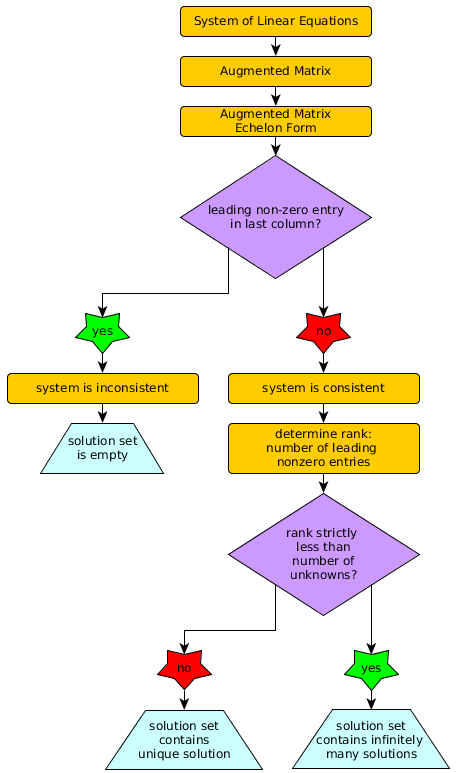
\includegraphics[scale=.4]{./diagrams/echelon.png}
  \end{figure}
\end{frame}

\begin{frame}
  \frametitle{Echelon Form Exercises}
  {\ubung} Determine the number of solutions for the following echelon
  forms.
  \begin{equation}
    \label{eq:uababohk}
    \left[
      \begin{array}{cccc}
        5 & -3 & 1 & 4 \\
        0 & -\frac{7}{5} & \frac{4}{5} & \frac{1}{5} \\
        0 & 0 & 0 & -2
      \end{array}\right]\hspace{.25in}\left[
      \begin{array}{cccc}
        2 & \pi & 4 & 3 \\
        0 & 5 & 6 & -13 \\
        0 & 0 & 0 & 0
      \end{array}\right]\hspace{.25in}\left[
      \begin{array}{cccc}
        3 & e^{2} & -1 & 12 \\
        0 & 1 & 0 & 6 \\
        0 & 0 & 4 & 0
      \end{array}\right]\notag
  \end{equation}
  \begin{equation}
    \label{eq:oataequa}
    \left[
      \begin{array}{cccc}
        3 & e^{2} & -1 & 12 \\
        0 & 1 & 0 & 6
      \end{array}\right]\hspace{.5in}\left[
      \begin{array}{cccc}
        3 & e^{2} & -1 & 12 \\
        0 & 1 & 0 & 6 \\
        0 & 0 & 3 & -8 \\
        0 & 0 & 0 & 14 \\
        0 & 0 & 0 & 0
      \end{array}\right]\notag
  \end{equation}
\end{frame}

\begin{frame}
  \frametitle{End of Lesson}
Next Lesson: Vectors
\end{frame}

\end{document}

